%%
%% Author: gdidot
%% 7/13/18
%%

% Preamble
\documentclass[11pt, a4paper, pdftex]{article}

% Packages
\usepackage[a4paper,top=3cm,bottom=2cm,left=3cm,right=3cm,marginparwidth=1.75cm,head=61pt]{geometry}
\usepackage{a4wide}
\usepackage[french]{babel}
\usepackage[utf8]{inputenc}
\usepackage{graphicx}
\usepackage{fancyhdr}
\usepackage{lastpage}
\usepackage[T1]{fontenc}
\usepackage[toc,page]{appendix}
\usepackage{caption}
\usepackage[hidelinks, colorlinks = true, urlcolor = blue, linkcolor = black]{hyperref}

\renewcommand{\appendixtocname}{Annexes}
\renewcommand{\appendixpagename}{Annexes}

\newcommand{\info}{\texttt}

% Document
\begin{document}

    %Custom style

    \pagestyle{fancy}
    \renewcommand{\sectionmark}[1]{\markright{\thesection\ #1}}
    \renewcommand{\subsectionmark}[1]{}

    \fancypagestyle{pagedegarde}{%
        \pagenumbering{gobble}
        \fancyhead[L]{
\includegraphics[height=1.5cm]{../assets/logo_istic.png}}
        \fancyhead[R]{
\includegraphics[height=1.5cm]{../assets/logo_univ_rennes1.png}}
        \renewcommand{\headrulewidth}{0pt}
        \fancyfoot[L]{
\includegraphics[height=1.5cm]{../assets/logo_irisa.png}}
        \fancyfoot[R]{
\includegraphics[height=1.5cm]{../assets/logo_diverse.png}}
    }

    \fancypagestyle{document}{%
        \pagenumbering{arabic}
        \renewcommand{\headrulewidth}{1pt}
        \fancyhead[L]{
\includegraphics[height=1.0cm]{../assets/logo_istic.png}}
        \fancyhead[C]{\rightmark}
        \fancyhead[R]{
\includegraphics[height=1.0cm]{../assets/logo_univ_rennes1.png}}
        \fancyfoot[C]{\thepage/\pageref{LastPage}}
    }

    %Info pour maketitle
    \title{Rapport de Stage: \\ Portage de la librairie Malai pour le WEB}
    \author{Gwendal \bsc{Didot}}

    %Setup de la page de garde
    \maketitle
    \thispagestyle{pagedegarde}
    \begin{center}
        \vspace{0.25cm} Master 1 Informatique spécialisation Sécurité, Système et Réseaux \\ à l'ISTIC, Université Rennes 1 \\
        \vspace{0.25cm} Encadré par M. Arnaud \bsc{Blouin} \\
        \vspace{0.25cm} Enseignant suiveur M. David \bsc{Gross-Amblard} \\
        \vspace{0.25cm} Stage réalisé du \date{15 mai 2018} au \date{31 août 2018} \\ \vspace{0.25cm} dans l'équipe DiverSE \\ des laboratoires INRIA/IRISA \\ sur le campus de Beaulieu, Rennes
    \end{center}


    \newpage
    \clearpage
    \setcounter{page}{1}
    \pagestyle{document}
    \section*{Remerciements}\label{sec:remerciement}
    \paragraph{}
    Je tiens à remercier Monsieur Arnaud \bsc{Blouin}, mon maître de stage, pour sa patience, sa pédagogie, et pour m'avoir permis de découvrir l'environnement WEB et ses technologies. \\
    Je remercie aussi tous les membres de l'équipe DiverSE pour leur accueil durant ce stage.
    \newpage

    \tableofcontents

    \newpage

    \section{Introduction}\label{sec:introduction}
        \paragraph{}
            Les interfaces utilisateur sont une partie essentielle des logiciels ou matériels informatiques.
            Une bonne interface utilisateur est ce qui permet d'avoir une bonne expérience utilisateur.

        \paragraph{}
            Dans le cadre de mon Master 1 à l'Istic, j'ai souhaité réaliser ce stage car il me permettait de toucher à une partie de l'informatique que je n'avais
            qu'effleuré durant mon cursus universitaire.
            De plus, j'ai toujours été intéressé de savoir comment était créée une librairie informatique.
            J'ai voulu intégrer l'équipe DiverSE des laboratoires INRIA/IRISA car sa façon de travailler me paraissait proche des méthodes utilisées dans les entreprises.
            La perspective de pouvoir travailler sur des technologies d'avenir m'a aussi motivé pour faire ce stage.

        \paragraph{}
            Dans un premier temps, nous décrirons rapidement les laboratoires INRIA et IRISA, nous verrons ensuite plus en détail les objectifs de mon stage,
            enfin, nous présenterons le travail réalisé durant le stage, afin de dresser un bilan de celui-ci.
    \newpage
    \section{Présentation de l'entreprise}\label{sec:presentr}
    \vspace{1cm}
    \subsection{IRISA et Inria}\label{subsec:irisa}
        \paragraph{}
            L'Institut de Recherche en Informatique et Systèmes Aléatoires (IRISA) est un laboratoire de recherche en informatique, automatique,
            traitement du signal et des images et en robotique. Il regroupe des membres de nombreux organismes de recherche, dont l'INRIA\@.
            L'Institut National de Recherche en Informatique et en Automatique (INRIA) est un établissement de recherche public en sciences du numérique,
            sous la tutelle du Ministère de l'Enseignement supérieur et de la Recherche et celui de l'Économie et des Finances.
            Il est séparé en différents centres de recherches autonomes à travers la France.
            Les domaines de recherche de ces laboratoires sont variés, comme le génie logiciel, la sécurité informatique, l'algorithmique ou encore la réalité virtuelle et le traitements des images.
            Ces domaines sont répartis au sein de l'IRISA parmi 38 équipes de recherche.
    \vspace{1cm}
    \subsection{DiverSE}\label{subsec:diverse}
             \paragraph{}
                L'équipe de recherche DiverSE est membre de l'IRISA et de l'INRIA. Son domaine de recherche se porte sur l'ingénierie logiciel, où elle développe de nouveaux modèles,
                méthodes et théories permettant de répondre aux besoins causés par la diversification des façons de penser, déployer et faire évoluer les systèmes fortement axés sur les logiciels.
                Cette équipe a pour avantage d'avoir des liens étroits avec l'industrie, ce qui se retrouve dans la façon de travailler de ses membres.
    \newpage
    \section{Objectif du stage}\label{sec:objsta}
    \vspace{1cm}
        \subsection{Présentation de Malai}\label{subsec:premal}
            \paragraph{}
                Les interfaces utilisateurs sont un composant essentiel pour un logiciel, mais actuellement les moyens donnés au développeur pour réaliser
                une interface sont assez rudimentaires, demandant un développement très bas niveau, et n'offre pas de moyen de facilement réutiliser du code.
                Pour remédier à ce problème, Malai à été créé pour permettre au développeur d'interface utilisateur de pouvoir le faire bien plus facilement, et avec un gain de temps non négligeable.
    \vspace{1cm}
        \subsection{Objectif Principal}\label{subsec:objsta}
            \paragraph{}
                Ayant vocation à être utilisé par tous développeurs d'interfaces utilisateur, Malai se doit d'être présent pour l'environnement WEB, du simple site html et javascript aux frameworks les plus complexes.
                Cependant Malai n'était pour le moment développé que pour l'environnement applicatif, avec JavaFX. Le but du stage était donc de porter le code Java de Malai
                vers Typescript, ainsi que réaliser des applications permettant de montrer les avantages de MalaiTS (la version WEB de Malai) par rapport aux standards actuels.
            \paragraph{}
                Avec le développement des applications de tests de MalaiTS, j'ai rapidement rencontré des problèmes dus à la structure de l'implémentation de Malai pour Java.
                Cela s'explique par le fait que l'environnement Java et l'environnement WEB sont différents.
                Le stage s'est donc aussi porté sur la recherche de solutions aux problèmes spécifiques à l'environnement WEB rencontrés avec MalaiTS\@.
    \newpage
    \section{Travail réalisé}\label{sec:trarea}
        Pour pouvoir comprendre le travail effectué, nous suggérons de lire l'annexe~\ref{sec:presmalaitech} qui donne une explication technique du fonctionnement de MalaiTS\@.

        \subsection{État initial}\label{subsec:travinit}
            \paragraph{}
                Ce stage ayant pour but le portage de Malai vers l'environnement WEB, les différents principes était déjà existants, je n'avais donc qu'à réécrire le code de Malai en TypeScript, ou l'adapter si besoin.
                De plus le c\oe ur du fonctionnement de MalaiTS avait déjà été codé par mon maître de stage Arnaud Blouin.

        \subsection{Portage vers Typescript}\label{subsec:mainjob}
            \paragraph{}
                Le système principal ayant déjà été implémenté, j'ai principalement réalisé le portage des interactions utilisateurs par défaut, celles qui sont proposées avec MalaiTS\@.
                J'ai aussi rajouté plusieurs des binders par défaut et, suite à des observations effectuées lors de tests, j'ai modifié certaines mécaniques
                des binders pour les rendre compatibles avec l'environnement WEB\@.
                J'ai aussi fait le portage des tests de Malai pour les interactions utilisateur en les adaptant pour l'environnement de test de MalaiTS\@.

        \subsection{Utilisation de MalaiTS}\label{subsec:travexem}
            \paragraph{}
                Pour montrer l'intérêt d'utiliser MalaiTS pour le développement d'interface utilisateur, j'ai commencé le développement de deux applications servant d'exemple.
                Une application de création de FSM réalisée avec le framework Angular, ce qui a permis de montrer certaines limitations dans la conception de MalaiTS,
                mais qui a aussi permis de confirmer que MalaiTS est utilisable pour créer une interface utilisateur dans l'environnement WEB\@.
                L'autre application est une application de calendrier utilisant la technologie React, ce qui m'a mené à créer MalaiTS-react, une version spécifique de MalaiTS car React a un comportement particulier.

    \newpage
    \section{Bilan du stage}\label{sec:bilsta}
        \subsection{État finale}\label{subsec:etatfin}
            \paragraph{}
                A la fin du stage, une grande partie du portage a été effectuée.
                Toutes les interactions utilisateurs sont présentes et sont testées.
                Une partie des binders ont été implémentés, et sont également testés.
                La dernière grande partie du portage à réaliser est le portage des commandes par défaut.
                Les deux applications servant d'exemple montrent que MalaiTS peut être utilisé pour créer des interfaces utilisateur d'application WEB, la version de développement de MalaiTS est d'ailleurs disponible sur npm sous le nom \info{org.malai.ts-dev}.
                Il serait d'ailleurs intéressant de créer une application servant d'exemple uniquement en HTML/JavaScript/CSS pour observer l'intérêt de MalaiTS dans ce cas de figure.

        \subsection{Compétences acquises}\label{subsec:compacq}
            \paragraph{}
                Je pense que ce stage m'a été bénéfique, car le WEB n'étant pas un des principaux sujets de mon cursus universitaire, il m'a permis de découvrir les technologies du WEB, les frameworks populaires et leur fonctionnement.
                Grâce à ce stage j'ai acquis des connaissances sur le modèle Vue/Contrôleur/Donnée utilisé pour créer des interfaces utilisateurs, l'utilisation des frameworks servant à créer des interfaces utilisateurs pour le WEB\@.
                Les compétences que j'ai acquis durant mon cursus m'ont permis de comprendre rapidement les besoins de ce stage, et m'ont permis de répondre efficacement à ces besoins.
                Durant le stage, j'ai découvert le principe de l'intégration continue et j'ai appris des fonctionnalités avancées de git et GitHub ainsi que les différents gitflow\footnote{Ensembles de bonnes pratiques à respecter quand on utilise le gestionnaire de version Git, voir le \href{https://guides.github.com/introduction/flow/}{GitHub Flow} ou le \href{https://about.gitlab.com/2014/09/29/gitlab-flow/}{GitLab Flow}, le plus abouti selon pour moi.} existants,
                et je pense que ces compétences sont essentielles pour un développeur et il serait intéressant de les voir enseignées dès la première année de licence.

    \newpage

    \section{Résumé[FR]/Summary[EN]}\label{sec:resume}
        \subsection{Français}\label{subsec:franc}
            \paragraph{}
                Ce stage est réalisé dans le cadre du stage obligatoire de Master 1 Sécurité, Systèmes et Réseaux de l'ISTIC\@.
                J'ai réalisé ce stage sous la supervision de M. Arnaud \bsc{Blouin}, dans l'équipe de recherche DiverSE à l'IRISA\@.
                J'ai réalisé le portage d'une partie de la librairie Malai en Java vers la version WEB MalaiTS en TypeScript, le système principal ayant déjà été porté par mon maître de stage.
                J'ai aussi mis en place différentes application WEB utilisant Malai pour leur interface utilisateur, servant d'exemple pour valider le fonctionnement de MalaiTS dans un environnement WEB\@.

            \paragraph{}
                Dans ce rapport j'explique succinctement le fonctionnement de Malai (voir annexe~\ref{sec:presmalaitech}), mais je ne rentre pas dans les détails, vous pouvez obtenir plus d'informations sur le dépôt GitHub de \href{https://github.com/arnobl/Malai}{Malai}.

        \subsection{English}\label{subsec:eng}
            \paragraph{}
                This internship is performed as the mandatory internship of the ISTIC first year Master of Security, Systems and Networks university degree.
                My supervisor is M. Arnaud \bsc{Blouin} and the internship takes place in the DiverSE research team at IRISA\@.
                I realise the port of a part of Malai library in Java to the WEB version MalaiTS in TypeScript, the core of the library was already port by my supervisor.
                I also create WEB applications with MalaiTS to serve as an example and proof-of-concept.

            \paragraph{}
                In this report I explain the basics of how Malai work (see appendice~\ref{sec:presmalaitech} in French), but I do not go into details. You can refer to the GitHub of \href{https://github.com/arnobl/Malai}{Malai} for further information.

    \newpage

    \fancyhead[C]{\huge Annexes}

    \begin{appendices}
        \section{Présentation technique de MalaiTS}\label{sec:presmalaitech}
            Le principe général de MalaiTS peu être séparé en 3 groupes:
            \begin{itemize}
                \vspace{0.2cm}
                \item Interaction utilisateur : Les interactions utilisateur correspondent aux actions de l'utilisateur sur les éléments (widgets) de l'interface utilisateur.
                Par exemple un clic sur un bouton ou un glisser-déposer (Drag and Drop) sont des interactions utilisateur courantes.
                Ces interactions peuvent être décrites sous la forme d'une machine à état fini (Finish State Machine ou FSM), et c'est ainsi que MalaiTS décrit les interactions.
                Les interactions utilisateur les plus courantes sont présentes dans MalaiTS, mais il est possible pour un développeur de créer des interactions personnalisées. \par
                \vspace{0.5cm}
                    \begin{minipage}{\linewidth}
                        \centering
                        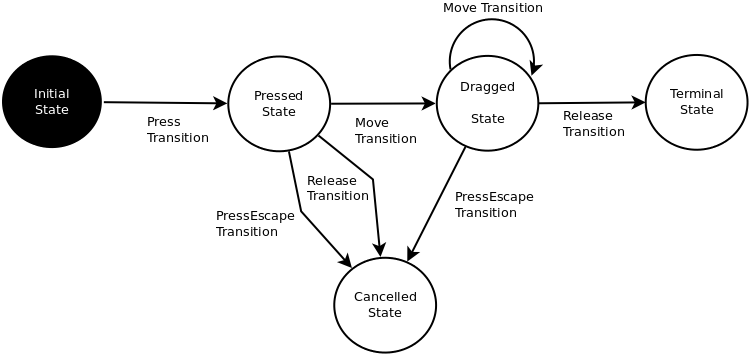
\includegraphics[height=6.0cm]{../assets/DnD.png}
                        \captionof{figure}{FSM du Drag and Drop}
                    \end{minipage}
                \vspace{0.5cm}
                \item Commande : Les commandes sont des actions qui seront appelées quand l'interaction utilisateur qui leur est liée sera effectuée.
                MalaiTS possède les commandes de base courantes, mais permet de très facilement implémenter des commandes personnalisées.
                \vspace{0.2cm}
                \item Binder : Ce système est l'intérêt principal de Malai, il permet de lier une commande avec une interaction, tout en pouvant paramétrer le binder.
                Comme par exemple en donnant une condition pour que la commande soit effectuée, ou bien en effectuant une commande à chaque fois que l'interaction utilisateur est mise à jour.
            \end{itemize}

    \end{appendices}

\end{document}
